\section{Complications}

[I have a note: TC1: Track local state ???]

\subsection{Release, Acquire, and SC Access}

Write $\Q{}$ as $\Q{\mSC}$ and introduce $\Q{\mRA}$.

$\Q{\mSC}$ implies $\Q{\mRA}$.


Access modes can be encoded in the independency relation, indexing labels by
$\amode$, but the extra flexibility of the logic is necessary for \armeight{}
(see \textsection\ref{sec:internal}).  Using independency, one would also
need another way to define completed pomsets.  Finally, this use of
independency is incompatible with fork (see \textsection\ref{sec:co}).

[visualization.  Labels to be turned off later in macros]
\begin{gather*}
  \hbox{\begin{tikzinline}[node distance=1.5em]
      \event{a1}{\DW{x}{0}}{}
      \raevent{a2}{\DW[\mRA]{x}{1}}{right=of a1}
      \scevent{a3}{\DR[\mSC]{x}{0}}{right=of a2}
      \xform{a4}{\aForm}{right=of a3}
      \sync{a2}{a3}
      \xo{a3}{a4}
      \wk{a1}{a2}
    \end{tikzinline}}
\end{gather*}

\subsection{ARM Compilation: Internal Acquires}
\label{sec:internal}
Downgrading acquires/Anton example: $\Dx{\aLoc}$

% $\D$ implies $\Dx{\aLoc}$

We write $[\aForm/\D]$ for the substitution that performs
$[\aForm/\Dx{\aLoc}]$ for every $\aLoc$.


Our solution allows executions that are not allowed under \armeight{} since
we do not insist that the local relaxed write is actually read from.  This
may seem counterintuitive, but we don't see a local way to be more precise.


\subsection{ARM Compilation: Read-read dependencies}
Control dependencies into reads as in MP with release on right and control
dependency on left.

$\RW$ implies $\lnot\RO$ and 
$\RO$ implies $\lnot\RW$.


\subsection{Putting it together}


If we move coherence to independency (and use fork-join), we have the
following, assuming that each register occurs at most once.
\begin{align*}
  \QS{}{\mSC}&=\Q{\mSC}
  &\QS{}{\mRA}&=\Q{\mRA}
  &\QS{}{\mRLX}&=\Qx{\aLoc}
  \\
  \QL{}{\mSC}&=\Q{\mSC}
  &\QL{}{\mRA}&=\Qw{\aLoc}
  &\QL{}{\mRLX}&=\Qw{\aLoc}
  \\
  \DS{\aLoc}{\mSC}{\aForm}&=\aForm[\FALSE/\D]
  &\DS{\aLoc}{\mRA}{\aForm}&=\aForm[\FALSE/\D]
  &\DS{\aLoc}{\mRLX}{\aForm}&=\aForm[\TRUE/\Dx{\aLoc}] 
  \\
  \DL{\aLoc}{\mSC}&=\Dx{\aLoc}
  &\DL{\aLoc}{\mRA}&=\Dx{\aLoc}
  &\DL{\aLoc}{\mRLX}&=\TRUE
\end{align*}

$\QS{}{\mRLX}=\TRUE$ and otherwise $\QS{}{\amode}=\Q{\amode}$.

$\QL{}{\mSC}=\Q{\mSC}$ and otherwise $\QL{}{\amode}=\TRUE$.

$\DS{\aLoc}{\mRLX}{\aForm}=\aForm[\TRUE/\Dx{\aLoc}]$ and otherwise
$\DS{\aLoc}{\amode}{\aForm}=\aForm[\FALSE/\D]$. 

$\DL{\aLoc}{\mRLX}=\TRUE$ and otherwise $\DL{\aLoc}{\amode}=\Dx{\aLoc}$.

\begin{definition}$\phantom{\;}$\par
  $\QS{}{\mRLX}=\TRUE$ and otherwise $\QS{}{\amode}=\Q{\amode}$.

  $\QL{}{\mSC}=\Q{\mSC}$ and otherwise $\QL{}{\amode}=\TRUE$.

  \smallskip

  \noindent
  If $\aPS \in \sSTORE[\amode]{\aLoc}{\aExp}$ then
  \begin{enumerate}
  \item[\ref{S1}--\ref{S2})] as before,
  \item[\ref{S3})]
    $\labelingForm(\aEv)$ implies
    \begin{math}
      \aExp{=}\aVal
      \land \RW
      \land \QS{}{\amode}
    \end{math},
  \item[\ref{S4})]
    $\aTr[\bEvs](\aForm)$ implies 
    \begin{math}
      \aExp{=}\aVal
      \land \DS{\aLoc}{\amode}{\aForm[\aExp/{\aLoc}]}
    \end{math},
  \item[\ref{S5})]
    $\aTr[\emptyset](\aForm)$ implies 
    \begin{math}
      \lnot\Q{\mRA}
      \land \DS{\aLoc}{\amode}{\aForm[\aExp/{\aLoc}]}
    \end{math}
  \end{enumerate}

  \noindent
  If $\aPS \in \sLOAD[\amode]{\aReg}{\aLoc}$ then
  \begin{enumerate}
  \item[\ref{L1}--\ref{L2})] as before,
  \item[\ref{L3})] $\labelingForm(\aEv)$ implies
    \begin{math}
      \RO
      \land \QL{}{\amode}
    \end{math},
  \item[\ref{L4})]
    $\aTr[\bEvs](\aForm)$ implies
    \begin{math}
      (\aVal{=}\aReg)
      \limplies \aForm[\aReg/{\aLoc}]
    \end{math}
  \item[\ref{L5})] 
    $\aTr[\emptyset](\aForm)$ implies
    \begin{math}
      \DL{\aLoc}{\amode}
      \land \lnot\Q{\mRA}
      \land
      (\RW
      \limplies (\aVal{=}\aReg\lor\aLoc{=}\aReg) 
      \limplies \aForm[\aReg/{\aLoc}]
      ).
    \end{math}
  \end{enumerate}  
\end{definition}

\subsection{Coherence}
\label{sec:co}

$\Q{\mSC}$ implies $\Q{\mRA}$ implies $\Qx{\aLoc}$ implies $\Qw{\aLoc}$

\begin{itemize}
\item Coherence respects program order: $\Qx{\aLoc}$
\item Drop read-read coherence: $\Qw{\aLoc}$ (Required for CSE without
  alias analysis over read only code, not required by hardware)
\end{itemize}

It is also possible to put coherence in the independency relation, in which
case, the semantics of $;$ includes the following.
\begin{enumerate}
  \setcounter{enumi}{\value{pomsetXSemiCount}}
\item
  \label{seq-reorder} if $\bEv\in\aEvs_1$ and $\aEv\in\aEvs_2$ either $\bEv<\SB0\aEv$ or $a\reorder\labeling_2(\aEv)$.
\end{enumerate}
One must be careful, however, due to \emph{inconsistency}.
Consider that \texttt{x=0;x=1} should not have completed pomset with only $\DWP{x}{0}$.

\eqref{seq-reorder} does not do the right thing with fork either.  If you
want to enforce coherence this way then you need to use fork-join as the
sequential combinator, rather than fork.

\begin{figure*}
  \begin{center}
    \begin{minipage}{0.905\textwidth}
      \noindent
If $\aPS \in \sSTORE[\amode]{\cExp}{\aExp}$ then
$(\exists\cVal:\aEvs\fun\Val)$
$(\exists\aVal:\aEvs\fun\Val)$
$(\exists\cForm:\aEvs\fun\Formulae)$
\begin{enumerate}
\item[\ref{S1})] if $\cForm_\bEv\land\cForm_\aEv$ is satisfiable then $\bEv=\aEv$,
\item[\ref{S2})] $\labelingAct(\aEv) = \DWREF{\cVal_\aEv}{\aVal_\aEv}$,
\item[\ref{S3})] 
  $\labelingForm(\aEv)$ implies
  \begin{math}
    \cForm_\aEv
    \land \QS{\REF{\cVal_\aEv}}{\amode}
    % \land \RW
    \land \cExp{=}\cVal_\aEv
    \land \aExp{=}\aVal_\aEv
  \end{math},
  % where
  % $\QS{}{\mRLX}=\QxREF{\cVal_\aEv}$ and otherwise $\QS{}{\amode}=\Q{\amode}$, % for $\amode\neq\mRLX$,
\item[\ref{S4})]
  \begin{math}
    (\forall\dVal)
    (\forall\aEv\in\aEvs\cap\bEvs)
  \end{math}
  $\aTr{\bEvs}{\bForm}$ \;implies \,
  \begin{math}
    \cForm_\aEv
    \limplies (\cExp{=}\dVal)
    \limplies \PBR{
      %(\QwREF{\dVal} \limplies \aExp{=}\aVal_\aEv) \land
      \bForm
      [\aExp/\REF{\dVal}]
      \DS{\REF{\dVal}}{\amode}
      [(\QwREF{\dVal}\land\aExp{=}\aVal)/\QwREF{\dVal}]
    }
  \end{math},
\item[\ref{S5})] %if 
  % \begin{math}
  %   (\forall\aEv\in\bEvs)(\cForm \textimplies
  %   \lnot\cForm_\aEv)
  % \end{math}
  % then
  \begin{math}
    (\forall\dVal)
  \end{math}
  $\aTr{\cEvs}{\bForm}$ implies
  \begin{math}
    (\!\not\exists\aEv\in\aEvs\cap\cEvs \suchthat \cForm_\aEv)
    \limplies (\cExp{=}\dVal)
    \limplies \PBR{
      % \lnot\QwREF{\dVal} \land
      \bForm
      [\aExp/\REF{\dVal}]
      \DS{\REF{\dVal}}{\amode}
      [\FALSE/\QS{\REF{\dVal}}{\amode}]
    }.
  \end{math}
  % \\ where 
  % $\DS{}{\mRLX}{}=[\TRUE/\DxREF{\dVal}]$ and otherwise
  % $\DS{}{\amode}{}=[\FALSE/\D]$. % for $\amode\neq\mRLX$.
\end{enumerate}
% \item if $\amode=\mRLX$ then
%   $\labelingForm(\aEv)$ implies
%   \begin{math}
%     \cForm_\aEv
%     \land \cExp{=}\cVal_\aEv
%     \land \aExp{=}\aVal_\aEv
%     \land \RW
%     \land \QxREF{\cVal_\aEv},
%   \end{math}
% \item if $\amode\neq\mRLX$ then
%   $\labelingForm(\aEv)$ implies
%   \begin{math}
%     \cForm_\aEv
%     \land \cExp{=}\cVal_\aEv
%     \land \aExp{=}\aVal_\aEv
%     \land \RW
%     \land \Q{},
%   \end{math}
% \item if
%   $\aEv\in\bEvs$
%   and
%   $\amode=\mRLX$ then
%   \begin{math}
%     (\forall\dVal)
%   \end{math}
%   $\aTr{\bEvs}{\bForm}$ implies 
%   \begin{math}
%     \cForm_\aEv
%     \limplies (\cExp{=}\dVal)
%     \limplies \PBRbig{
%     (\QwREF{\dVal} \limplies \aExp{=}\aVal_\aEv)
%     \land \bForm[\aExp/\REF{\dVal}][\TRUE/\DxREF{\dVal}]
%   }
%   \end{math}
% \item if
%   $\aEv\in\bEvs$
%   and
%   $\amode\neq\mRLX$ then
%   \begin{math}
%     (\forall\dVal)
%   \end{math}
%   $\aTr{\bEvs}{\bForm}$ implies 
%   \begin{math}
%     \cForm_\aEv
%     \limplies (\cExp{=}\dVal)
%     \limplies \PBRbig{
%     (\QwREF{\dVal} \limplies \aExp{=}\aVal_\aEv)
%     \land \bForm[\aExp/\REF{\dVal}][\FALSE/\D]
%   }
%   \end{math}
% \item if 
%   \begin{math}
%     (\forall\aEv\in\bEvs)(\cForm \textimplies
%     \lnot\cForm_\aEv)
%   \end{math}
%   and $\amode=\mRLX$ 
%   then
%   \begin{math}
%     (\forall\dVal)
%   \end{math}
%   $\aTr{\bEvs}{\bForm}$ implies 
%   \begin{math}
%     \cForm
%     \limplies (\cExp{=}\dVal)
%     \limplies \PBRbig{
%     \lnot\QwREF{\dVal}
%     \land \bForm[\aExp/\REF{\dVal}][\TRUE/\DxREF{\dVal}]
%   }
%   \end{math}
% \item if 
%   \begin{math}
%     (\forall\aEv\in\bEvs)
%     (\cForm \textimplies \lnot\cForm_\aEv)
%   \end{math}
%   and $\amode\neq\mRLX$ 
%   then
%   \begin{math}
%     (\forall\dVal)
%   \end{math}
%   $\aTr{\bEvs}{\bForm}$ implies 
%   \begin{math}
%     \cForm
%     \limplies (\cExp{=}\dVal)
%     \limplies \PBRbig{
%     \lnot\QwREF{\dVal}
%     \land \bForm[\aExp/\REF{\dVal}][\FALSE/\D]
%   }
%   \end{math}

\noindent
If $\aPS \in \sLOAD[\amode]{\aReg}{\cExp}$ then
$(\exists\cVal:\aEvs\fun\Val)$
$(\exists\aVal:\aEvs\fun\Val)$
$(\exists\cForm:\aEvs\fun\Formulae)$
% $(\forall\uReg{\aEv}\in\uRegs{\aEvs})$
\begin{enumerate}
\item[\ref{L1})] if $\cForm_\bEv\land\cForm_\aEv$ is satisfiable then $\bEv=\aEv$,
\item[\ref{L2})] $\labelingAct(\aEv) = \DRREF{\cVal_\aEv}{\aVal_\aEv}$,
\item[\ref{L3})] $\labelingForm(\aEv)$ implies
  \begin{math}
    \cForm_\aEv
    \land \QL{\REF{\cVal_\aEv}}{\amode}
    % \land \RO
    \land \cExp{=}\cVal_\aEv
  \end{math},
  % where    
  % $\QL{}{\mSC}=\Q{\mSC}$ and otherwise $\QL{}{\amode}=\QwREF{\cVal_\aEv}$, % for $\amode\neq\mRLX$,
\item[\ref{L4})]
  \begin{math}
    (\forall\dVal)
    (\forall\aEv\in\aEvs\cap\bEvs)
  \end{math}
  $\aTr{\bEvs}{\bForm}$ implies
  \begin{math}
    \cForm_\aEv
    \limplies (\cExp{=}\dVal)
    \limplies (\aVal_\aEv{=}\uReg{\aEv})
    \limplies \bForm[\uReg{\aEv}/\aReg]%[\uReg{\aEv}/\REF{\dVal}]
  \end{math},
  \makebox[5.75cm]{}
\item[\ref{L5})] 
  \begin{math}
    (\forall\dVal)
    (\forall\aEv\in\aEvs\setminus\cEvs)
  \end{math}
  $\aTr{\cEvs}{\bForm}$ implies
  \begin{math}
    \cForm_\aEv
    \limplies (\cExp{=}\dVal)
    \limplies \PBR{        
      %\lnot\QxREF{\dVal}\land
      \DL{\REF{\dVal}}{\amode} \land
      (\RW
      \limplies (\aVal_\aEv{=}\uReg{\aEv}\lor\REF{\dVal}{=}\uReg{\aEv}) 
      \limplies
      \bForm
      [\uReg{\aEv}/\aReg]%[\uReg{\aEv}/\REF{\dVal}]
      [\FALSE/\QL{\REF{\dVal}}{\amode}]
      )
    }      
  \end{math},
\item[\ref{L6})] % if 
  % \begin{math}
  %   (\forall\aEv\in\bEvs)(\cForm \textimplies
  %   \lnot\cForm_\aEv)
  % \end{math}
  % then
  \begin{math}
    (\forall\dVal)
    (\forall\bReg)
  \end{math}
  $\aTr{\dEvs}{\bForm}$  implies 
  \begin{math}
    (\!\not\exists\aEv\in\aEvs \suchthat \cForm_\aEv)
    \limplies (\cExp{=}\dVal)
    \limplies \PBR{        
      %\lnot\QxREF{\dVal} \land
      \DL{\REF{\dVal}}{\amode} \land
      \bForm
      [\bReg/\aReg]%[\bReg/\REF{\dVal}]
      [\FALSE/\QL{\REF{\dVal}}{\amode}]
    }.
  \end{math}
  % \\ where $\DL{}{\mRLX}=\TRUE$ and otherwise $\DL{}{\amode}=\DxREF{\dVal}$.
  % Recall that $\uRegs{\bEvs}=\{\uReg{\aEv}\mid\aEv\in\bEvs\}$.
\end{enumerate}  
% \item if $\amode=\mRLX$ and $\bEv\notin\bEvs$ then
%   \begin{math}
%     (\forall\dVal)
%   \end{math}
%   $\aTr{\bEvs}{\bForm}$ implies
%   \begin{math}
%     \cForm_\bEv
%     \limplies (\cExp{=}\dVal)
%     \limplies \PBRbig{
%     (
%     \RW
%     \limplies (\aVal{=}\uReg{\bEv}\lor\aLoc{=}\uReg{\bEv}) 
%     \limplies \bForm[\uReg{\bEv}/\aReg][\uReg{\bEv}/\REF{\dVal}]
%     )
%     \land \lnot\QxREF{\dVal}
%   }
%     \phantom{\land\; \Dx{\dVal}}
%   \end{math}
% \item if $\amode\neq\mRLX$ and $\bEv\notin\bEvs$ then
%   \begin{math}
%     (\forall\dVal)
%   \end{math}
%   $\aTr{\bEvs}{\bForm}$ implies
%   \begin{math}
%     \cForm_\bEv
%     \limplies (\cExp{=}\dVal)
%     \limplies \PBRbig{
%     (
%     \RW
%     \limplies (\aVal{=}\uReg{\bEv}\lor\aLoc{=}\uReg{\bEv}) 
%     \limplies \bForm[\uReg{\bEv}/\aReg][\uReg{\bEv}/\REF{\dVal}]
%     )
%     \land \lnot\QxREF{\dVal}
%     \land \Dx{\dVal}
%   }
%   \end{math}

\noindent
If $\aPS \in \sTHREAD{\aPSS}$ then
$(\exists\aPS_1\in\aPSS)$
\begin{enumerate}
\item[\ref{T1})]
  $\aEvs=\aEvs_1$,
\item[\ref{T2})]
  $\labelingAct(\aEv) = \labelingAct_1(\aEv)$,
\item[\ref{T3})]
  $\labelingForm(\aEv)$ implies
  $\labelingForm_1(\aEv) [\TRUE/\Qr{*}][\TRUE/\Qw{*}][\TRUE/\Qsc][\TRUE/\RW]$ if $\labelingAct_1(\aEv)$ is a write,
  \\
  $\labelingForm(\aEv)$ implies
  $\labelingForm_1(\aEv) [\TRUE/\Qr{*}][\TRUE/\Qw{*}][\TRUE/\Qsc][\FALSE/\RW]$ otherwise.
\end{enumerate}  

      % \noindent
If $\aPS \in \sSTORE[\amode]{\cExp}{\aExp}$ then
$(\exists\cVal:\aEvs\fun\Val)$
$(\exists\aVal:\aEvs\fun\Val)$
$(\exists\cForm:\aEvs\fun\Formulae)$
\begin{enumerate}
\item if $\cForm_\bEv\land\cForm_\aEv$ is satisfiable then $\bEv=\aEv$,
\item $\labelingAct(\aEv) = \DWREFP{\cVal_\aEv}{\aVal_\aEv}$,
\item 
  $\labelingForm(\aEv)$ implies
  \begin{math}
    \cForm_\aEv
    \land \cExp{=}\cVal_\aEv
    \land \aExp{=}\aVal_\aEv
    \land \RW
    \land \Qmode{\amode}
  \end{math},
  where
  $\Qmode{\mRLX}=\QxREF{\cVal_\aEv}$ and otherwise $\Qmode{\amode}=\Q{\amode}$, % for $\amode\neq\mRLX$,
\item
  \begin{math}
    (\forall\dVal)
  \end{math}
  if
  $\bEv\in\bEvs$
  then
  $\aTr{\bEvs}{\aForm}$ implies 
  \begin{math}
    \cForm_\bEv
    \limplies (\cExp{=}\dVal)
    \limplies \PBRbig{
      (\QwREF{\dVal} \limplies \aExp{=}\aVal_\bEv)
      \land \aForm [\aExp/\REF{\dVal}]\Dmode{\amode}
    }
  \end{math},
\item %if 
  % \begin{math}
  %   (\forall\bEv\in\bEvs)(\cForm \textimplies
  %   \lnot\cForm_\bEv)
  % \end{math}
  % then
  \begin{math}
    (\forall\dVal)
  \end{math}
  $\aTr{\bEvs}{\aForm}$ implies 
  \begin{math}
    (\not\exists\bEv\in\bEvs.\; \cForm_\bEv)
    \limplies (\cExp{=}\dVal)
    \limplies \PBR{
      \lnot\QwREF{\dVal}
      \land \aForm [\aExp/\REF{\dVal}]\Dmode{\amode}
    }
  \end{math},
  \\ where 
  $\Dmode{\mRLX}=[\TRUE/\DxREF{\dVal}]$ and otherwise
  $\Dmode{\amode}=[\FALSE/\D]$. % for $\amode\neq\mRLX$.
\end{enumerate}
% \item if $\amode=\mRLX$ then
%   $\labelingForm(\aEv)$ implies
%   \begin{math}
%     \cForm_\aEv
%     \land \cExp{=}\cVal_\aEv
%     \land \aExp{=}\aVal_\aEv
%     \land \RW
%     \land \QxREF{\cVal_\aEv},
%   \end{math}
% \item if $\amode\neq\mRLX$ then
%   $\labelingForm(\aEv)$ implies
%   \begin{math}
%     \cForm_\aEv
%     \land \cExp{=}\cVal_\aEv
%     \land \aExp{=}\aVal_\aEv
%     \land \RW
%     \land \Q{},
%   \end{math}
% \item if
%   $\bEv\in\bEvs$
%   and
%   $\amode=\mRLX$ then
%   \begin{math}
%     (\forall\dVal)
%   \end{math}
%   $\aTr{\bEvs}{\aForm}$ implies 
%   \begin{math}
%     \cForm_\bEv
%     \limplies (\cExp{=}\dVal)
%     \limplies \PBRbig{
%     (\QwREF{\dVal} \limplies \aExp{=}\aVal_\bEv)
%     \land \aForm[\aExp/\REF{\dVal}][\TRUE/\DxREF{\dVal}]
%   }
%   \end{math}
% \item if
%   $\bEv\in\bEvs$
%   and
%   $\amode\neq\mRLX$ then
%   \begin{math}
%     (\forall\dVal)
%   \end{math}
%   $\aTr{\bEvs}{\aForm}$ implies 
%   \begin{math}
%     \cForm_\bEv
%     \limplies (\cExp{=}\dVal)
%     \limplies \PBRbig{
%     (\QwREF{\dVal} \limplies \aExp{=}\aVal_\bEv)
%     \land \aForm[\aExp/\REF{\dVal}][\FALSE/\D]
%   }
%   \end{math}
% \item if 
%   \begin{math}
%     (\forall\bEv\in\bEvs)(\cForm \textimplies
%     \lnot\cForm_\bEv)
%   \end{math}
%   and $\amode=\mRLX$ 
%   then
%   \begin{math}
%     (\forall\dVal)
%   \end{math}
%   $\aTr{\bEvs}{\aForm}$ implies 
%   \begin{math}
%     \cForm
%     \limplies (\cExp{=}\dVal)
%     \limplies \PBRbig{
%     \lnot\QwREF{\dVal}
%     \land \aForm[\aExp/\REF{\dVal}][\TRUE/\DxREF{\dVal}]
%   }
%   \end{math}
% \item if 
%   \begin{math}
%     (\forall\bEv\in\bEvs)
%     (\cForm \textimplies \lnot\cForm_\bEv)
%   \end{math}
%   and $\amode\neq\mRLX$ 
%   then
%   \begin{math}
%     (\forall\dVal)
%   \end{math}
%   $\aTr{\bEvs}{\aForm}$ implies 
%   \begin{math}
%     \cForm
%     \limplies (\cExp{=}\dVal)
%     \limplies \PBRbig{
%     \lnot\QwREF{\dVal}
%     \land \aForm[\aExp/\REF{\dVal}][\FALSE/\D]
%   }
%   \end{math}

\noindent
If $\aPS \in \sLOAD[\amode]{\aReg}{\cExp}$ then
$(\exists\cVal:\aEvs\fun\Val)$
$(\exists\aVal:\aEvs\fun\Val)$
$(\exists\cForm:\aEvs\fun\Formulae)$
% $(\forall\uReg{\aEv}\in\uRegs{\aEvs})$
\begin{enumerate}
\item if $\cForm_\bEv\land\cForm_\aEv$ is satisfiable then $\bEv=\aEv$,
\item $\labelingAct(\aEv) = \DRREFP{\cVal_\aEv}{\aVal_\aEv}$,
\item $\labelingForm(\aEv)$ implies
  \begin{math}
    \cForm_\aEv
    \land \cExp{=}\cVal_\aEv
    \land \RO
    \land \Qmode{\amode}
  \end{math},
  where    
  $\Qmode{\mSC}=\Q{\mSC}$ and otherwise $\Qmode{\amode}=\QwREF{\cVal_\aEv}$, % for $\amode\neq\mRLX$,
\item
  \begin{math}
    (\forall\dVal)
  \end{math}
  if $\bEv\in\bEvs$ then
  $\aTr{\bEvs}{\aForm}$ implies
  \begin{math}
    \cForm_\bEv
    \limplies (\cExp{=}\dVal)
    \limplies (\aVal{=}\uReg{\bEv})
    \limplies \aForm[\uReg{\bEv}/\aReg][\uReg{\bEv}/\REF{\dVal}]
  \end{math},
  \makebox[4.4cm]{}
\item 
  \begin{math}
    (\forall\dVal)
  \end{math}
  if $\bEv\notin\bEvs$ then
  $\aTr{\bEvs}{\aForm}$ implies
  \begin{math}
    \cForm_\bEv
    \limplies (\cExp{=}\dVal)
    \limplies \PBRbig{        
      \Dmode{\amode}
      \land \lnot\QxREF{\dVal}
      \land
      (\RW
      \limplies (\aVal{=}\uReg{\bEv}\lor\aLoc{=}\uReg{\bEv}) 
      \limplies \aForm[\uReg{\bEv}/\aReg][\uReg{\bEv}/\REF{\dVal}]
      )
    }      
  \end{math},
\item % if 
  % \begin{math}
  %   (\forall\bEv\in\bEvs)(\cForm \textimplies
  %   \lnot\cForm_\bEv)
  % \end{math}
  % then
  \begin{math}
    (\forall\dVal)
    (\forall\bReg)
  \end{math}
  $\aTr{\bEvs}{\aForm}$ implies 
  \begin{math}
    (\not\exists\bEv\in\bEvs.\; \cForm_\bEv)
    \limplies (\cExp{=}\dVal)
    \limplies \PBR{        
      \Dmode{\amode}
      \land \lnot\QxREF{\dVal}
      \land
      \limplies \aForm[\bReg/\aReg][\bReg/\REF{\dVal}]
    }      
  \end{math},
  \\ where $\Dmode{\mRLX}=\TRUE$ and otherwise $\Dmode{\amode}=\Dx{\dVal}$.
  Recall that $\uRegs{\bEvs}=\{\uReg{\bEv}\mid\bEv\in\bEvs\}$.
\end{enumerate}  
% \item if $\amode=\mRLX$ and $\bEv\notin\bEvs$ then
%   \begin{math}
%     (\forall\dVal)
%   \end{math}
%   $\aTr{\bEvs}{\aForm}$ implies
%   \begin{math}
%     \cForm_\bEv
%     \limplies (\cExp{=}\dVal)
%     \limplies \PBRbig{
%     (
%     \RW
%     \limplies (\aVal{=}\uReg{\bEv}\lor\aLoc{=}\uReg{\bEv}) 
%     \limplies \aForm[\uReg{\bEv}/\aReg][\uReg{\bEv}/\REF{\dVal}]
%     )
%     \land \lnot\QxREF{\dVal}
%   }
%     \phantom{\land\; \Dx{\dVal}}
%   \end{math}
% \item if $\amode\neq\mRLX$ and $\bEv\notin\bEvs$ then
%   \begin{math}
%     (\forall\dVal)
%   \end{math}
%   $\aTr{\bEvs}{\aForm}$ implies
%   \begin{math}
%     \cForm_\bEv
%     \limplies (\cExp{=}\dVal)
%     \limplies \PBRbig{
%     (
%     \RW
%     \limplies (\aVal{=}\uReg{\bEv}\lor\aLoc{=}\uReg{\bEv}) 
%     \limplies \aForm[\uReg{\bEv}/\aReg][\uReg{\bEv}/\REF{\dVal}]
%     )
%     \land \lnot\QxREF{\dVal}
%     \land \Dx{\dVal}
%   }
%   \end{math}

      % \noindent
If $\aPS \in \sSTORE[\amode]{\cExp}{\aExp}$ then
$(\exists\cVal:\aEvs\fun\Val)$
$(\exists\aVal:\aEvs\fun\Val)$
$(\exists\bForm:\aEvs\fun\Formulae)$
\begin{enumerate}
\item if $\bForm_\bEv\land\bForm_\aEv$ is satisfiable then $\bEv=\aEv$,
\item $\labelingAct(\aEv) = \DWREFP{\cVal_\aEv}{\aVal_\aEv}$,
\item 
  $\labelingForm(\aEv)$ implies
  \begin{math}
    \bForm_\aEv
    \land \cExp{=}\cVal_\aEv
    \land \aExp{=}\aVal_\aEv
    \land \RW
    \land \QS{}{\amode}
  \end{math},
\item
  \begin{math}
    (\forall\dVal)
  \end{math}
  if
  $\bEv\in\bEvs$
  then
  $\aTr[\bEvs](\aForm)$ implies 
  \begin{math}
    \bForm_\bEv
    \limplies (\cExp{=}\dVal)
    \limplies \PBRbig{
      \aExp{=}\aVal_\bEv
      \land \DS{\REF{\dVal}}{\amode}{\aForm[\aExp/\REF{\dVal}]}
    }
  \end{math},
\item 
  \begin{math}
    (\forall\dVal)
  \end{math}
  $\aTr[\bEvs](\aForm)$ implies 
  \begin{math}
    (\not\exists\bEv\in\bEvs.\; \bForm_\bEv)
    \limplies (\cExp{=}\dVal)
    \limplies \PBR{
      \lnot\Q{\mRA}
      \land \DS{\REF{\dVal}}{\amode}{\aForm[\aExp/\REF{\dVal}]}
    }.
  \end{math}
\end{enumerate}

\noindent
If $\aPS \in \sLOAD[\amode]{\aReg}{\cExp}$ then
$(\exists\cVal:\aEvs\fun\Val)$
$(\exists\aVal:\aEvs\fun\Val)$
$(\exists\bForm:\aEvs\fun\Formulae)$
\begin{enumerate}
\item if $\bForm_\bEv\land\bForm_\aEv$ is satisfiable then $\bEv=\aEv$,
\item $\labelingAct(\aEv) = \DRREFP{\cVal_\aEv}{\aVal_\aEv}$,
\item $\labelingForm(\aEv)$ implies
  \begin{math}
    \bForm_\aEv
    \land \cExp{=}\cVal_\aEv
    \land \RO
    \land \QL{}{\amode}
  \end{math},
\item
  \begin{math}
    (\forall\dVal)
  \end{math}
  if $\bEv\in\bEvs$ then
  $\aTr[\bEvs](\aForm)$ implies
  \begin{math}
    \bForm_\bEv
    \limplies (\cExp{=}\dVal)
    \limplies (\aVal{=}\uReg{\bEv})
    \limplies \aForm[\uReg{\bEv}/\aReg][\uReg{\bEv}/\REF{\dVal}]
  \end{math},
  \makebox[4.8cm]{}
\item 
  \begin{math}
    (\forall\dVal)
  \end{math}
  if $\bEv\notin\bEvs$ then
  $\aTr[\bEvs](\aForm)$ implies
  \begin{math}
    \bForm_\bEv
    \limplies (\cExp{=}\dVal)
    \limplies \PBRbig{        
      \DL{\REF{\dVal}}{\amode}
      \land \lnot\Q{\mRA}
      \land
      (\RW
      \limplies (\aVal{=}\uReg{\bEv}\lor\aLoc{=}\uReg{\bEv}) 
      \limplies \aForm[\uReg{\bEv}/\aReg][\uReg{\bEv}/\REF{\dVal}]
      )
    }      
  \end{math},
\item 
  \begin{math}
    (\forall\dVal)
    (\forall\bReg)
  \end{math}
  $\aTr[\bEvs](\aForm)$ implies 
  \begin{math}
    (\not\exists\bEv\in\bEvs.\; \bForm_\bEv)
    \limplies (\cExp{=}\dVal)
    \limplies \PBR{        
      \DL{\REF{\dVal}}{\amode}
      \land \lnot\Q{\mRA}
      \land
      \limplies \aForm[\bReg/\aReg][\bReg/\REF{\dVal}]
    }.
  \end{math}
\end{enumerate}  

    \end{minipage}
  \end{center}
  \caption{Full Semantics of Load and Store}
  \label{fig:full}
\end{figure*}    


Combining the features defined thus far, we have the following, assuming that
each register occurs at most once.

\begin{align*}
  \QS{\aLoc}{\mSC}&=\Q{\mSC}
  &\QS{\aLoc}{\mRA}&=\Q{\mRA}
  &\QS{\aLoc}{\mRLX}&=\Qx{\aLoc}
  \\
  \QL{\aLoc}{\mSC}&=\Q{\mSC}
  &\QL{\aLoc}{\mRA}&=\Qw{\aLoc}
  &\QL{\aLoc}{\mRLX}&=\Qw{\aLoc}
  \\
  \DS{\aLoc}{\mSC}{\aForm}&=\aForm[\FALSE/\D]
  &\DS{\aLoc}{\mRA}{\aForm}&=\aForm[\FALSE/\D]
  &\DS{\aLoc}{\mRLX}{\aForm}&=\aForm[\TRUE/\Dx{\aLoc}] 
  \\
  \DL{\aLoc}{\mSC}&=\Dx{\aLoc}
  &\DL{\aLoc}{\mRA}&=\Dx{\aLoc}
  &\DL{\aLoc}{\mRLX}&=\TRUE
\end{align*}

$\QS{\aLoc}{\mRLX}=\Qx{\aLoc}$ and otherwise $\QS{\aLoc}{\amode}=\Q{\amode}$.

$\QL{\aLoc}{\mSC}=\Q{\mSC}$ and otherwise $\QL{\aLoc}{\amode}=\Qw{\aLoc}$.

$\DS{\aLoc}{\mRLX}{\aForm}=\aForm[\TRUE/\Dx{\aLoc}]$ and otherwise
$\DS{\aLoc}{\amode}{\aForm}=\aForm[\FALSE/\D]$. 

$\DL{\aLoc}{\mRLX}=\TRUE$ and otherwise $\DL{\aLoc}{\amode}=\Dx{\aLoc}$.

\begin{definition}$\phantom{\;}$\par
  \noindent
  If $\aPS \in \sSTORE[\amode]{\aLoc}{\aExp}$ then
  \begin{enumerate}
  \item[\ref{S1}--\ref{S2})] as before,
  \item[\ref{S3})]
    $\labelingForm(\aEv)$ implies
    \begin{math}
      \aExp{=}\aVal
      \land \RW
      \land \QS{\aLoc}{\amode}
    \end{math},
  \item[\ref{S4})]
    $\aTr[\bEvs](\aForm)$ implies 
    \begin{math}
      (\Qw{\aLoc} \limplies \aExp{=}\aVal)
      \land \DS{\aLoc}{\amode}{\aForm[\aExp/{\aLoc}]}
    \end{math},
  \item[\ref{S5})]
    $\aTr[\emptyset](\aForm)$ implies 
    \begin{math}
      \lnot\Qw{\aLoc}
      \land \DS{\aLoc}{\amode}{\aForm[\aExp/{\aLoc}]}.
    \end{math}
  \end{enumerate}

  \noindent
  If $\aPS \in \sLOAD[\amode]{\aReg}{\aLoc}$ then
  \begin{enumerate}
  \item[\ref{L1}--\ref{L2})] as before,
  \item[\ref{L3})]
    $\labelingForm(\aEv)$ implies
    \begin{math}
      \RO
      \land \QL{\aLoc}{\amode}
    \end{math},
  \item[\ref{L4})]
    $\aTr[\bEvs](\aForm)$ implies
    \begin{math}
      (\aVal{=}\aReg)
      \limplies \aForm[\aReg/{\aLoc}]
    \end{math}
  \item[\ref{L5})] 
    $\aTr[\emptyset](\aForm)$ implies
    \begin{math}
      \DL{\aLoc}{\amode}
      \land \lnot\Qx{\aLoc}
      % \end{math}
      % \\
      % \begin{math}
      %   {}
      \land 
      (\RW
      \limplies (\aVal{=}\aReg\lor\aLoc{=}\aReg) 
      \limplies \aForm[\aReg/{\aLoc}]
      ).
    \end{math}
    % \item 
    %   $\aTr[\bEvs](\aForm)$ implies 
    %   \begin{math}
    %     (\not\exists\bEv\in\bEvs.\; \bForm)
    %     \limplies \PBR{        
    %     \DL{\aLoc}{\amode}
    %     \land \lnot\Qx{\aLoc}
    %     \land
    %     \limplies \aForm[\aReg/{\aLoc}]
    %   }      
    %   \end{math}
  \end{enumerate}  
\end{definition}



\section{Further Complications}

\subsection{Redundant Read Elimination}

Requires indexing to resolve nondeterminism.

\begin{gather*}
  \taglabel{TC2}
  \PR{x}{r}\SEMI
  \PR{x}{s}\SEMI
  \IF{r{=}s}\THEN \PW{y}{1}\FI
  \PAR
  x\GETS y
  \\
  \hbox{\begin{tikzinline}[node distance=1.5em]
      \event{a1}{\DR{x}{1}}{}
      \event{a2}{\DR{x}{1}}{right=of a1}
      \event{a3}{\DW{y}{1}}{right=of a2}
      % \po{a2}{a3}
      % \po[out=-20,in=-160]{a1}{a3}
      \event{b1}{\DR{y}{1}}{right=3em of a3}
      \event{b2}{\DW{x}{1}}{right=of b1}
      \rf{a3}{b1}
      \po{b1}{b2}
      \rf[out=169,in=11]{b2}{a2}
      \rf[out=169,in=11]{b2}{a1}
    \end{tikzinline}}
\end{gather*}
Precondition of $\DWP{y}{1}$ is $(r{=}s)$ in
\begin{math}
  \sem{\IF{r{=}s}\THEN y\GETS 1\FI}.
\end{math}
Predicate transformers for $\emptyset$ in $\sem{\PR{x}{r}}$ and $\sem{\PR{x}{s}}$ are
\begin{align*}
  \PREDP{(r{=}1 \lor r{=}x)\limplies\aForm[r/x]},
  \\
  \PREDP{(s{=}1 \lor s{=}x)\limplies\aForm[s/x]}.
\end{align*}
Combining the transformers, we have
\begin{displaymath}
  \PREDP{(r{=}1 \lor r{=}x)\limplies(s{=}1 \lor s{=}r)\limplies\aForm[s/x]}.
\end{displaymath}
Applying this to $(r{=}s)$, we have
\begin{displaymath}
  \PREDP{(r{=}1 \lor r{=}x)\limplies (s{=}1 \lor s{=}r)\limplies (r{=}s)},
\end{displaymath}
which is not a tautology.

Same problem occurs oopsla, where we have:
\begin{align*}
  \PREDP{\aForm[v/x,r] \land \aForm[x/r]},
  \\
  \PREDP{\aForm[v/x,s] \land \aForm[x/s]}.
\end{align*}
Combining the transformers, we have
\begin{displaymath}
  \PREDP{\aForm[v/x,r,s] \land \aForm [v/x,r][x/s] \land \aForm[x/r][v/x,s] \land \aForm[x/r,s]}.
\end{displaymath}
Applying this to $(r{=}s)$, we have
\begin{displaymath}
  \PREDP{v{=}v \land v{=}x \land x{=}v \land x{=}x},
\end{displaymath}
which is not a tautology.

The semantics here allows this by coalescing:
\begin{gather*}
  r\GETS x\SEMI
  s\GETS x\SEMI
  \IF{r{=}s}\THEN y\GETS 1\FI
  \PAR
  x\GETS y
  \\
  \hbox{\begin{tikzinline}[node distance=1.5em]
      \event{a1}{\DR{x}{1}}{}
      \event{a3}{\DW{y}{1}}{right=of a1}
      \event{b1}{\DR{y}{1}}{right=3em of a3}
      \event{b2}{\DW{x}{1}}{right=of b1}
      \rf{a3}{b1}
      \po{b1}{b2}
      \rf[out=169,in=11]{b2}{a1}
    \end{tikzinline}}
\end{gather*}

\subsection{If Closure}
Requires indexing to resolve nondeterminism.

IF closure/case analysis: $\psi_e$

\subsection{Address Calculation}

Do this after if closure, because problem with punning badly.

In $\sSTORE{}{}$:
\begin{enumerate}
\item[\ref{S1})] $\labelingAct\SB0(\aEv) = \DWP{\REF\cVal}{\aVal}$,
\item $\labelingForm\SB0(\aEv)$ implies $(\cExp{=}\cVal \land \aExp{=}\aVal)$,
\item $(\forall\dVal)$ $\aTr[\emptyset]\SB0(\aForm)$ implies $(\cExp{=}\dVal) \limplies \aForm[\aExp/\REF{\dVal}]$,
\item $(\forall\dVal)$ $\aTr[\bEvs]\SB0(\aForm)$ implies $(\cExp{=}\dVal) \limplies (\aExp{=}\aVal) \land \aForm[\aExp/\REF{\dVal}]$, 
\end{enumerate}

In $\sLOAD{}{}$:
\begin{enumerate}
\item $\labelingAct\SB0(\aEv) = \DRP{\REF{\cVal}}{\aVal}$,
\item $\labelingForm\SB0(\aEv)$ implies $(\cExp{=}\cVal)$,
\item $(\forall\dVal)$ $\aTr[\emptyset]\SB0(\aForm)$ implies
  $(\cExp{=}\dVal) \limplies (\aReg{=}\aVal\lor\aReg{=}\REF{\dVal})\limplies\aForm$,
\item $(\forall\dVal)$ $\aTr[\bEvs]\SB0(\aForm)$ implies
  $(\cExp{=}\dVal) \limplies (\aReg{=}\aVal)\limplies\aForm$, 
\end{enumerate}  

\subsection{Putting it together}

The full semantics of load and store is given in Figure \ref{fig:full}.
Recall that $\uRegs{\bEvs}=\{\uReg{\bEv}\mid\bEv\in\bEvs\}$.

% \subsection{Agda}
% \begin{figure*}
%   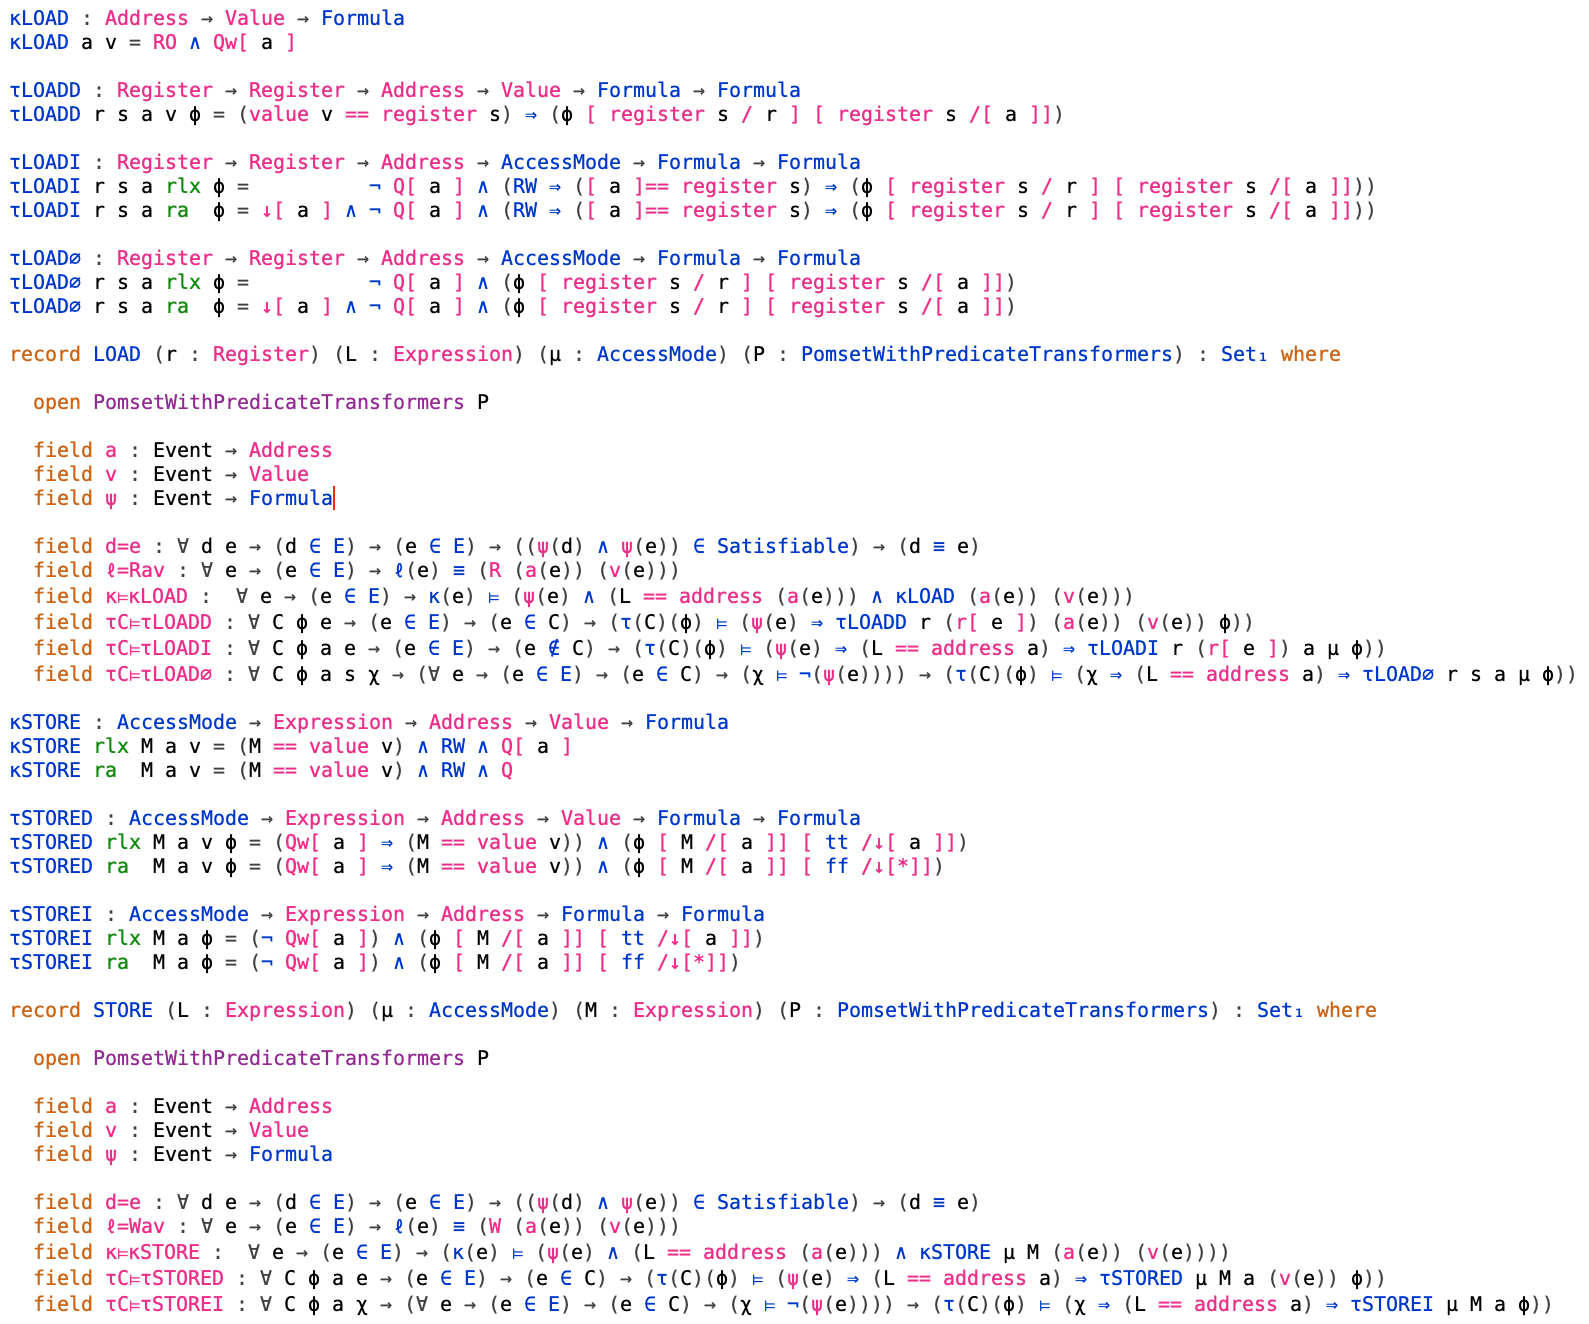
\includegraphics[width=\textwidth]{agda.png}
% \end{figure*}
